\documentclass{beamer}
\usetheme{metropolis}
\usepackage{graphicx}
\usepackage{amsmath}
\usepackage{url}

\def\rcurs{{\mbox{$\resizebox{.16in}{.08in}{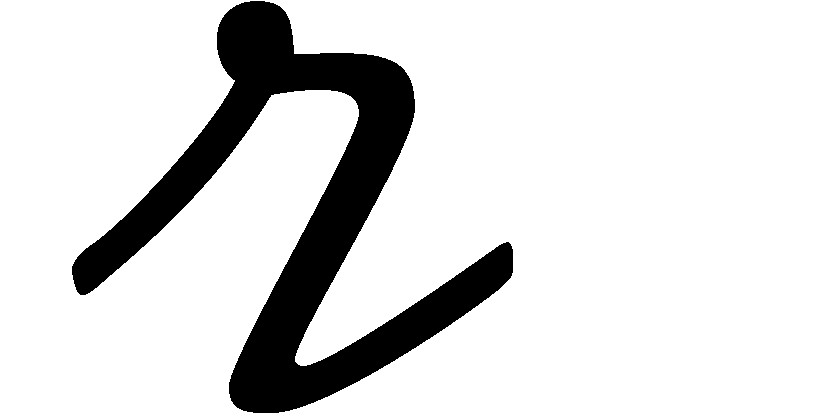
\includegraphics{ScriptR}}$}}}
\def\brcurs{{\mbox{$\resizebox{.16in}{.08in}{
\includegraphics{BoldR}}$}}}
\def\hrcurs{{\mbox{$\hat \brcurs$}}}

\title{Electromagnetc Theory: PHYS330}
\author{Jordan Hanson}
\institute{Whittier College Department of Physics and Astronomy}

\begin{document}
\maketitle

\section{Summary}

\begin{frame}{Week 4 Summary}
\begin{enumerate}
\item Atoms, polarizations, and dipole moments
\item $\vec{P}$, dipole per unit volume, and bound charges
\item $\vec{D}$, the electric displacement
\item Linear dielectrics
\end{enumerate}
\end{frame}

\section{Dipole Moment, and The Electric Field of a Dipole}

\begin{frame}{Dipole Moment, and The Electric Field of a Dipole}
From the multipole expansion, the monopole and dipole terms are (asynchronous video content):
\begin{align}
V(r,\theta)_{n=0} &= \frac{1}{4\pi\epsilon_0}\frac{\int_{all} \rho(\vec{r'})d\tau'}{r} \\
V(r,\theta)_{n=1} &= \frac{1}{4\pi\epsilon_0}\frac{\hat{r} \cdot \int_{all} \vec{r'} \rho(\vec{r'})d\tau'}{r^2} \\
\vec{p} &= \hat{r} \cdot \int_{all} \vec{r'} \rho(\vec{r'})d\tau'
\end{align}
\end{frame}

\begin{frame}{Dipole Moment, and The Electric Field of a Dipole}
Valid for any charge distribution, useful for getting far-field E-fields:
\begin{equation}
\boxed{
\vec{p} = \hat{r} \cdot \int_{all} \vec{r'} \rho(\vec{r'})d\tau'
}
\end{equation}
\begin{enumerate}
\item Discrete charge distribution example: asynch. video content
\item Continuous: ``similar'' to calculating the moment of inertia of a mass distribution (only it's linear vector, not $r'^2$).
\end{enumerate}
\end{frame}

\begin{frame}{Dipole Moment, and The Electric Field of a Dipole}
For a dipole, with no other charges ($\vec{p} = q\vec{d}$):
\begin{equation}
V_{n=1}(r,\theta) = \frac{\hat{r}\cdot\vec{p}}{4\pi\epsilon_0 r^2} \label{eq:dip}
\end{equation}
\begin{enumerate}
\item Using Eq. \ref{eq:dip}, calculate the electric field of a dipole in spherical coordinates.
\item Are there any regions for which the E-field is zero?
\item What happens when you set $\partial E/\partial \theta = 0$?
\item Recall that the energy density of a field is $u_E = \frac{1}{2}\epsilon_0 \vec{E} \cdot \vec{E}$.  For a given radius $R$, is the energy density higher at $\theta = 0$ or $\theta = \pi/2$?
\end{enumerate}
\textit{Breakout rooms.}
\end{frame}

\section{Atoms, polarizations, and dipole moments}

\begin{frame}{Atoms, polarizations, and dipole moments}
Suppose an external field $\vec{E}$ induces a dipole moment $\vec{p}$ in an atomic charge distribution:
\begin{equation}
\boxed{
\vec{p} = \alpha \vec{E}
}
\end{equation}
This statement is empirical, but it's true for ``ordinary'' field strengths: field isn't strong enough to ionize the atom.
\end{frame}

\begin{frame}{Atoms, polarizations, and dipole moments}
\textbf{What is the electric field a distance $d$ from the center of a uniformly charged sphere of radius $a$?} \textit{[Hint: use Gauss' law, and assume $\rho$ is constant in spherical coordinates].} \\ \vspace{6cm}
\end{frame}

\begin{frame}{Atoms, polarizations, and dipole moments}
Result:
\begin{equation}
E = \frac{1}{4\pi \epsilon_0}\frac{qd}{a^3}
\end{equation}
But then assume that $p = qd$, so
\begin{equation}
\alpha = 4\pi\epsilon_0 a^3
\end{equation}
\begin{figure}
\centering
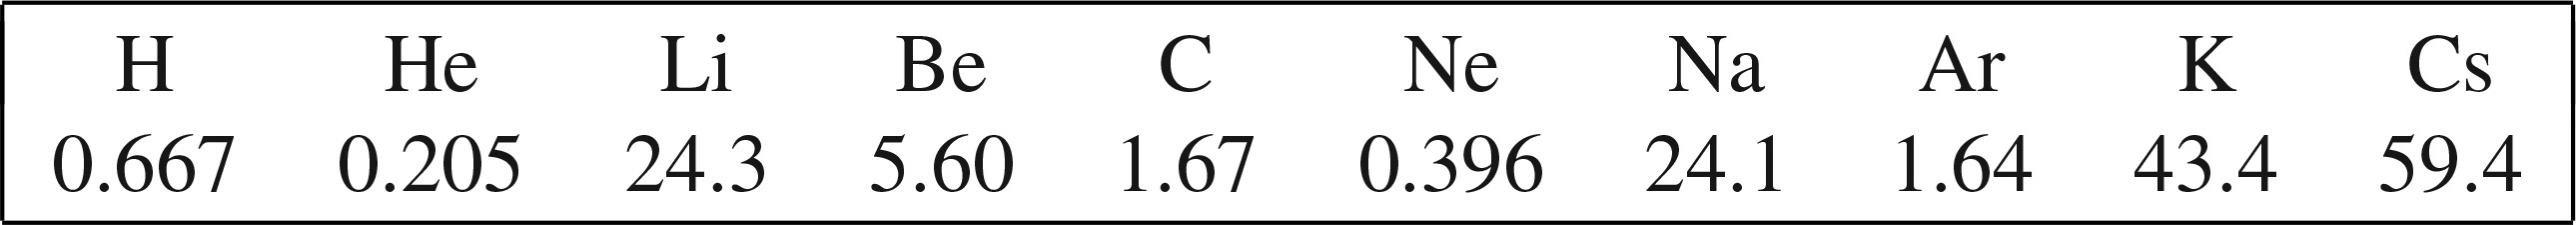
\includegraphics[width=10cm]{figures/tab4_1.jpg}
\caption{\label{tab:alpha} Do you understand the units of this table?  The numbers are quoted as $\alpha/4\pi\epsilon_0$, \textit{in units of $10^{-30}$ m$^3$.  What would they be in namometers cubed?}}
\end{figure}
The trouble is that we cannot easily measure the volume of an atom (realm of quantum mechanics).
\end{frame}

\begin{frame}{Atoms, polarizations, and dipole moments}
Molecules can also have a \textit{permanent} dipole moment: polar molecules.
\begin{figure}
\centering
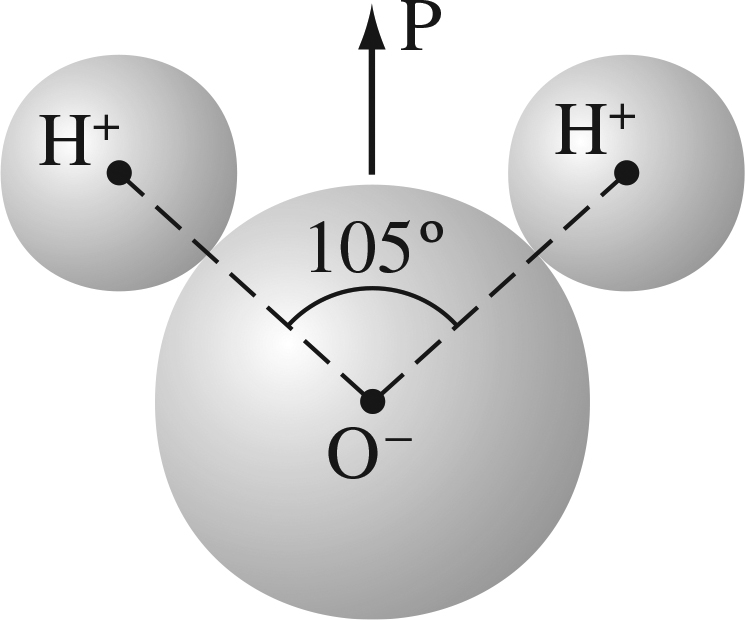
\includegraphics[width=3cm]{figures/4_4.jpg}
\caption{\label{fig:water} How would you calculate the dipole moment here?}
\end{figure}
Show that the torque on such a molecule in an external field is $\vec{\tau} = \vec{p} \times \vec{E}$ (Professor example).
\end{frame}

\begin{frame}{Atoms, polarizations, and dipole moments}
If you have (approximately) aligned polar molecules with an external field $\vec{E} = E_0 \hat{x}$, and then \textit{reverse} the direction of the field, in what direction is the torque?  Assume the dipole moments are in the xy-plane.
\begin{itemize}
\item A: $-\hat{z}$
\item B: $\hat{y}$
\item C: $\hat{z}$
\item D: The torque is zero
\end{itemize}
\end{frame}

\begin{frame}{Atoms, polarizations, and dipole moments}
In summary, there are two reasons there could be dipole moments within a material:
\begin{enumerate}
\item The atoms are \textit{stretched} and you get an $\alpha = 4\pi\epsilon_0 a^3$
\item The atoms or molecules are \textit{rotated} and you get a dipole moment $\vec{p}$ per atom/molecule.
\end{enumerate}
Macroscopically, it is easier to demonstrate the polar molecule effect: \url{https://youtu.be/riMrg_kO__w}
\end{frame}

\section{$\vec{P}$, dipole per unit volume, and bound charges}

\begin{frame}{$\vec{P}$, dipole per unit volume, and bound charges}
We need to understand the field of a polarized material.  Suppose we introduce the \textit{dipole moment per unit volume}, $\vec{P}$.
\begin{figure}
\centering
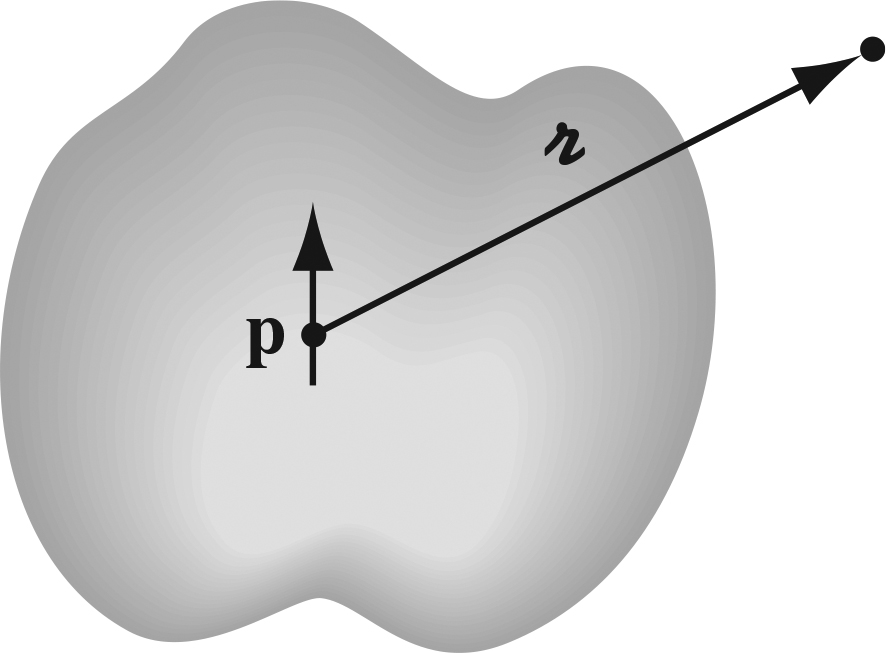
\includegraphics[width=6cm]{figures/4_8.jpg}
\caption{\label{fig:dipoleVol} The definition of the dipole moment per unit volume, and geometry.}
\end{figure}
\end{frame}

\begin{frame}{$\vec{P}$, dipole per unit volume, and bound charges}
This implies that
\begin{align}
\vec{p} &= \vec{P} d\tau' \\
V(r) &= \frac{1}{4\pi\epsilon_0}\frac{\vec{p} \cdot \hrcurs}{\rcurs^2} \\
V(r) &= \frac{1}{4\pi\epsilon_0}\int_{\mathcal{V}} \frac{\vec{P}(\vec{r'}) \cdot \hrcurs d\tau'}{\rcurs^2} \\
V(r) &= \frac{1}{4\pi\epsilon_0}\int_{\mathcal{V}} \vec{P}(\vec{r'}) \cdot \nabla \left( \frac{1}{\rcurs} \right) d\tau' \\
\nabla \cdot (f\vec{A}) &= f(\nabla \cdot \vec{A}) + \vec{A} \cdot \nabla(f) \\
V(r) &= \frac{1}{4\pi\epsilon_0} \left\lbrace \int_{\mathcal{V}} \nabla' \cdot \left( \frac{\vec{P}}{\rcurs} \right)d\tau' - \int_{\mathcal{V}} \frac{1}{\rcurs} \left(\nabla' \cdot \vec{P} \right) d\tau' \right\rbrace
\end{align}
\end{frame}

\begin{frame}{$\vec{P}$, dipole per unit volume, and bound charges}
\begin{align}
V(r) &= \frac{1}{4\pi\epsilon_0} \left\lbrace \int_{\mathcal{V}} \nabla' \cdot \left( \frac{\vec{P}}{\rcurs} \right)d\tau' - \int_{\mathcal{V}} \frac{1}{\rcurs} \left(\nabla' \cdot \vec{P} \right) d\tau' \right\rbrace \\
V(r) &= \frac{1}{4\pi\epsilon_0} \left\lbrace \oint_{\mathcal{S}} \left( \frac{\vec{P}}{\rcurs} \right) \cdot d\vec{a}' - \int_{\mathcal{V}} \frac{1}{\rcurs} \left(\nabla' \cdot \vec{P} \right) d\tau' \right\rbrace \\
d\vec{a}' &= da' \hat{n} \\
\sigma_b &= \vec{P} \cdot \hat{n} \\
\rho_b &= -\nabla \cdot \vec{P} \\
V(r) &= \frac{1}{4\pi\epsilon_0} \left\lbrace \oint_{\mathcal{S}} \frac{\sigma_b}{\rcurs} da'  - \int_{\mathcal{V}}  \frac{\rho_b}{\rcurs} d\tau' \right\rbrace \label{eq:bound}
\end{align}
The appearance of \textit{bound charge.}
\end{frame}

\begin{frame}{$\vec{P}$, dipole per unit volume, and bound charges}
\small
Suppose we have a sphere with uniform polarization in the z-direction (and it is constant).  The $\rho_b$ is zero because
\begin{itemize}
\item A: There is no bound charge inside a sphere.
\item B: The divergence of a constant is zero.
\item C: By symmetry.
\item D: Otherwise the integral over $\rho_b$ would diverge.
\end{itemize} 
\begin{figure}
\centering
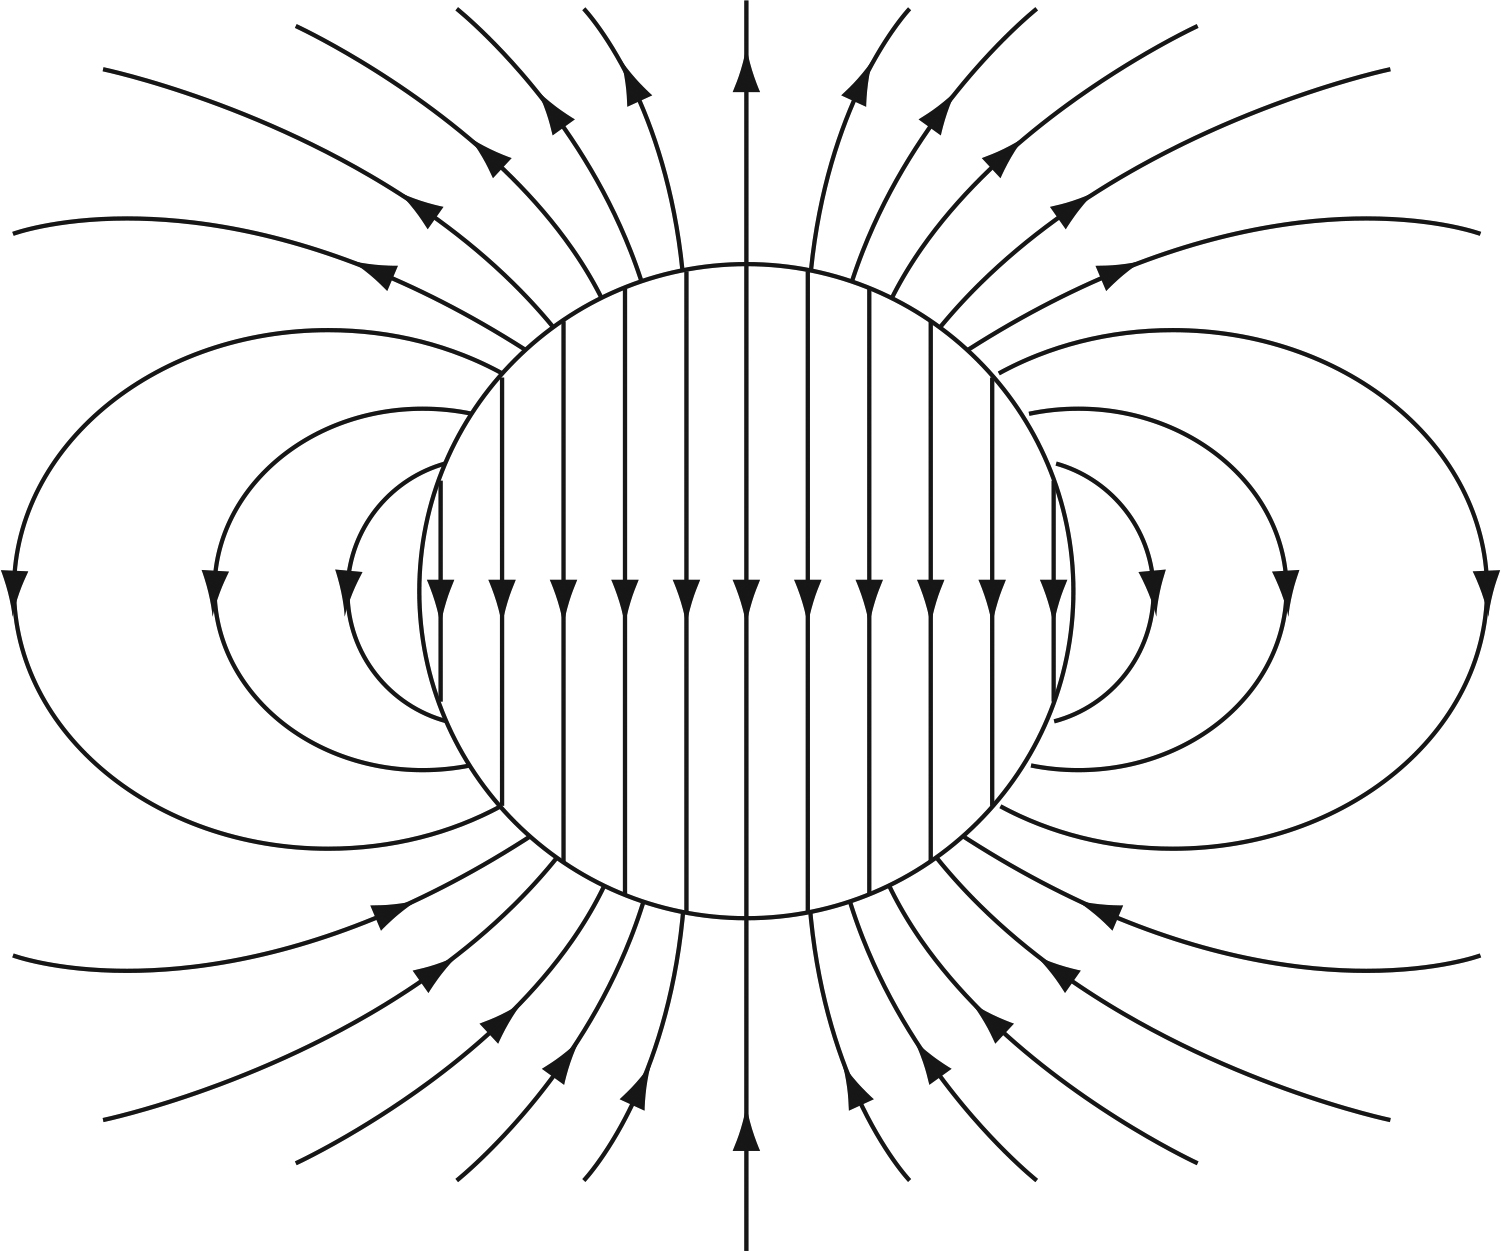
\includegraphics[width=3.5cm]{figures/4_10.jpg}
\caption{\label{fig:sigma} The uniformly polarized sphere. $\sigma_b = \vec{P} \cdot \hat{n} = P\cos\theta$.}
\end{figure}
\end{frame}

\begin{frame}{$\vec{P}$, dipole per unit volume, and bound charges}
\small
Think for a moment: in your own words, why do the field lines point in \textit{opposite} directions just inside and just outside the surface of the sphere?
\begin{figure}
\centering
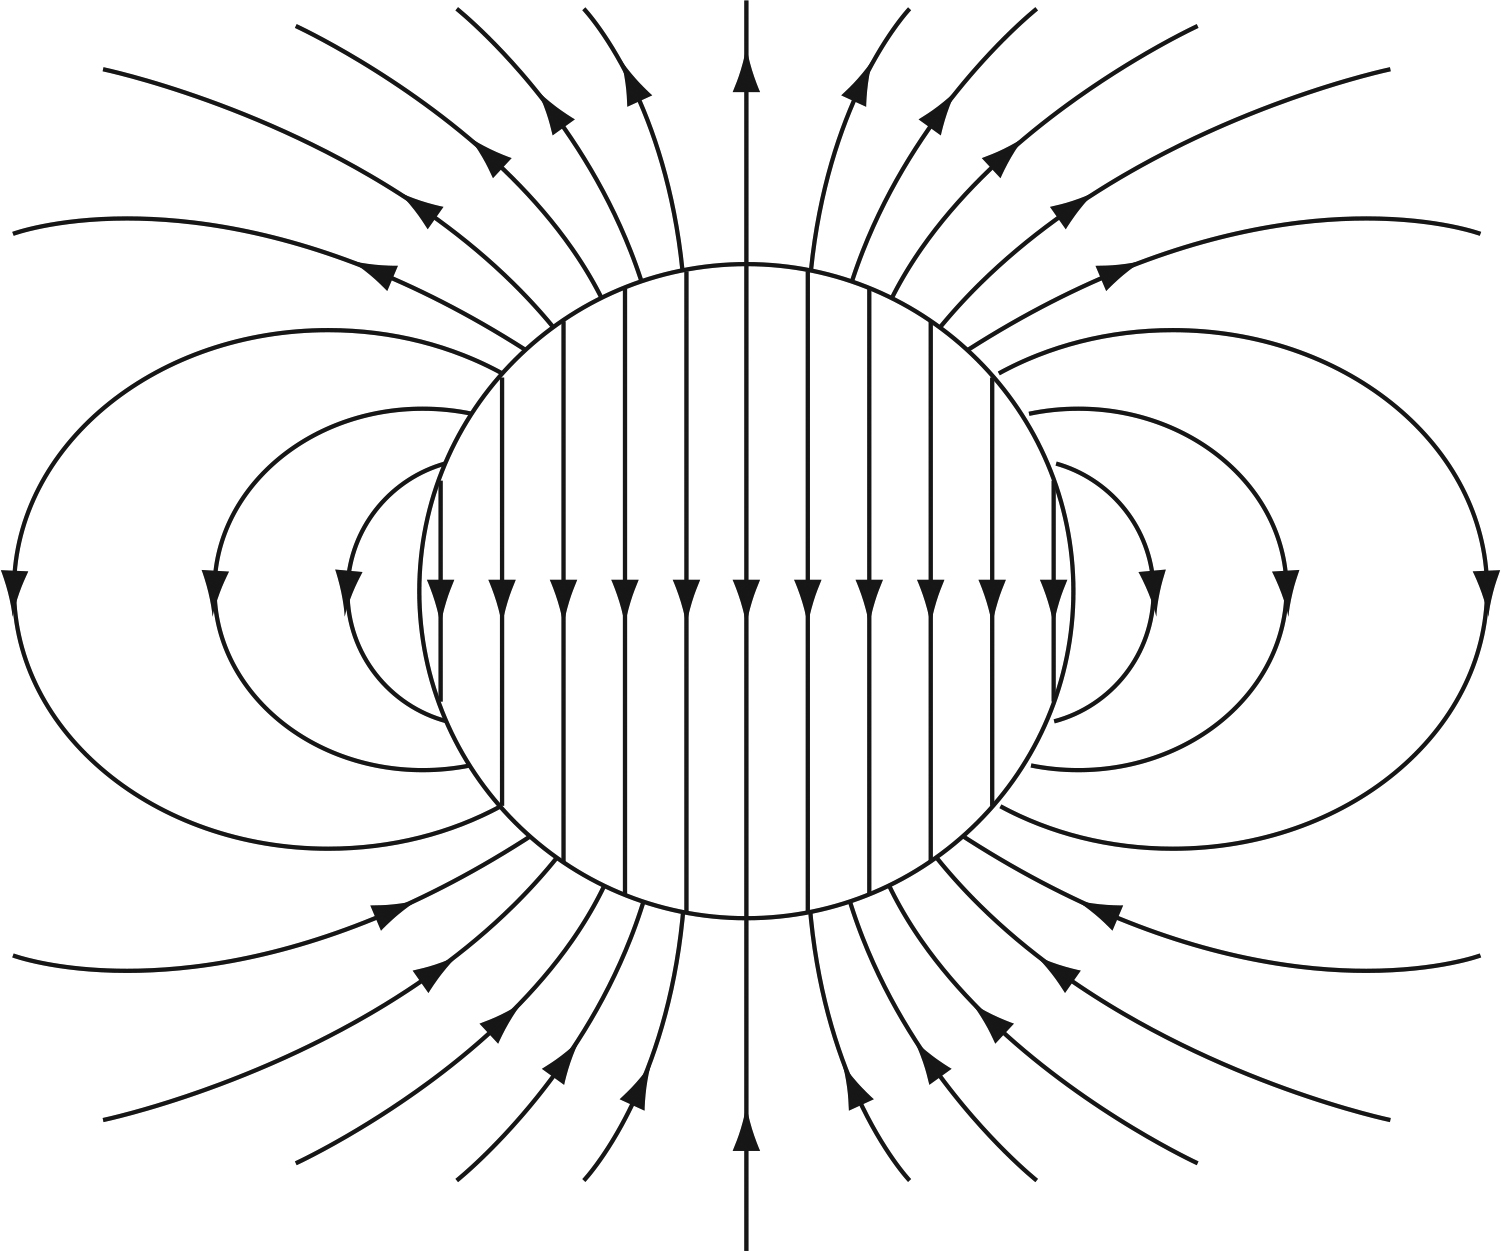
\includegraphics[width=3.5cm]{figures/4_10.jpg}
\caption{\label{fig:sigma2} The uniformly polarized sphere. $\sigma_b = \vec{P} \cdot \hat{n} = P\cos\theta$.}
\end{figure}
\end{frame}

\begin{frame}{$\vec{P}$, dipole per unit volume, and bound charges}
\begin{figure}
\centering
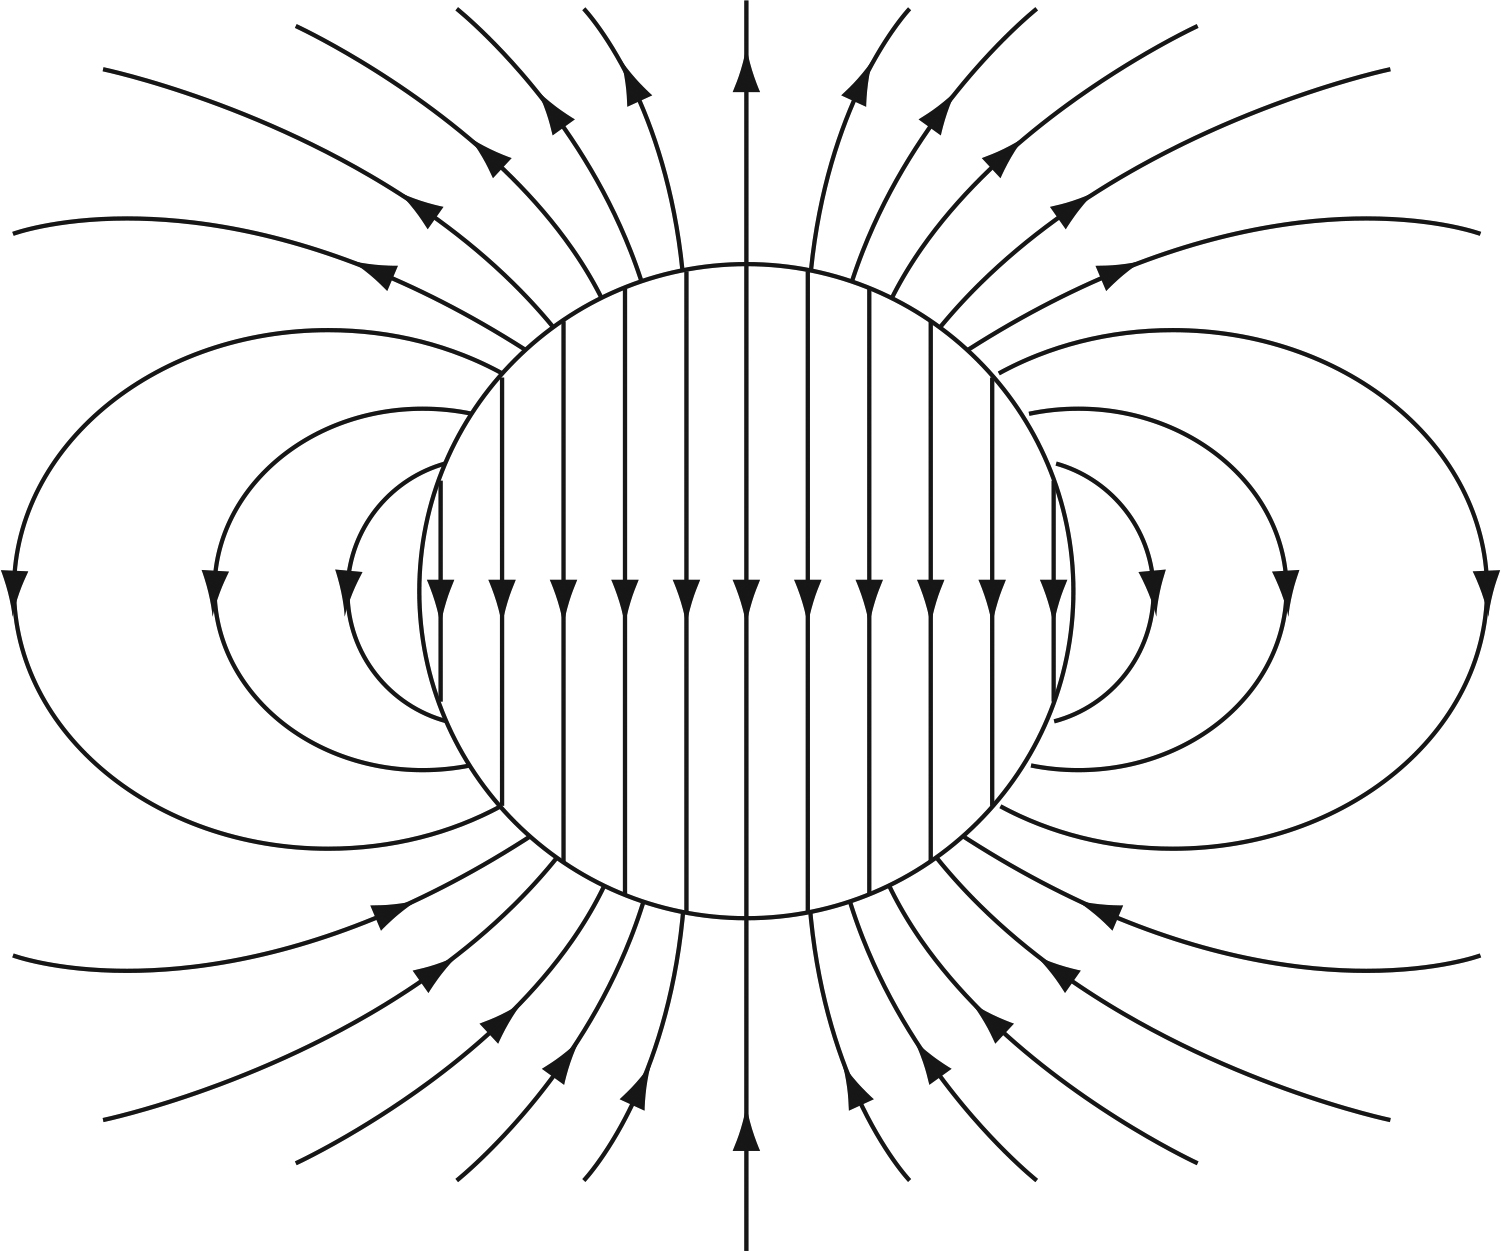
\includegraphics[width=3.5cm]{figures/4_10.jpg}
\caption{\label{fig:sigma3} The uniformly polarized sphere. $\sigma_b = \vec{P} \cdot \hat{n} = P\cos\theta$.}
\end{figure}
\begin{figure}
\centering
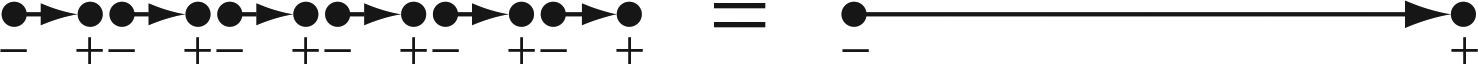
\includegraphics[width=7cm]{figures/4_11.jpg}
\caption{\label{fig:sigma4} Whenever you think of bound charge density versus surface charge density, think of this picture.}
\end{figure}
\end{frame}

\begin{frame}{$\vec{P}$, dipole per unit volume, and bound charges}
\textbf{Conceptual question:} Given Eq. \ref{eq:bound}, what is the potential due a disk of surface bound charge $\sigma_b$ at a point slightly above the surface? \textit{[Hint: if it helps, think of $\sigma_b = \vec{P_0} \cdot \hat{z}$, where $P_0$ is a constant.]}\\ \vspace{6cm}
\end{frame}

\section{$\vec{D}$, the electric displacement}

\section{Conclusion}

\begin{frame}{Week 4 Summary}
\begin{enumerate}
\item Atoms, polarizations, and dipole moments
\item $\vec{P}$, dipole per unit volume, and bound charges
\item $\vec{D}$, the electric displacement
\item Linear dielectrics
\end{enumerate}
\end{frame}

\end{document}
